\documentclass[../main.tex]{subfiles}
Vođeni idejom da projekat bude Web aplikaciju, idealan šablon za prezentovanje arhitekture sistema je Slojevita ahritektura (engl. Layered Pattern). \\
Slojevita arhitektura je idealan šablon jer nam omogućava: 
\begin{itemize}
    \item Paralelan rad na različitim slojevima arhitekture bez konflikta
    \item Omogućava fleksibilnost, održivosti i skalabilnost aplikacije
    \item Odvajanje Prezentacionog sloja od poslovne logike
    \item Deploy, ažuriranje, dodavanje novih feature-a na različitim slojevima i u različito vreme.
\end{itemize}


\begin{document}
\begin{figure}[!ht]
\begin{center}
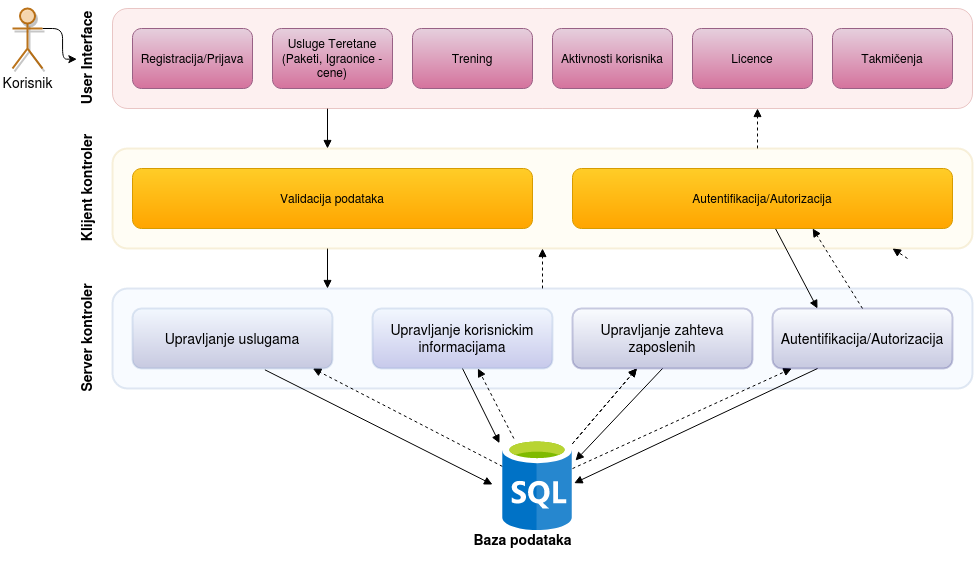
\includegraphics[scale=0.55]{sections/images/arhitektura_sistema.png}
\end{center}
\caption{Arhitektura sistema}
\label{fig:kontekst}
\end{figure}

\subsection{Opis arhitekture}
Slojevita arhitektura se sastoji od slojeva: 
\begin{itemize}
    \item Prezentacioni sloj (engl. User Interface - UI)
    \item Klijent kontroler
    \item Server kontroler
    \item Baza podataka
\end{itemize}

\textbf{Prezentacioni sloj} je sloj direktno dostupan korisniku sistema. Na slici su prikazane stranice koje će biti dostupne registrovanom korisniku i zaposlenom u sistemu. \\
Tehničku implementaciju ćemo izvršiti pomoću framework-a Angular. Kreiraćemo single-page aplikaciju koja će koristiti HTML, CSS i TypeScript. \\
\textbf{Klijent kontroler} je sloj koji će sadržati validaciju podataka koje je korisnik uneo i autentifikaciju/autorizaciju. 
Prilikom prijave korisnik, UI inicira poziv ka ekternom sistemu (kao npr. ForgeRock\footnote{https://www.forgerock.com/about-us}) i pribavlja token potreban za logovanje. Zatim se pravi request ka Server kotroleru. U sloju Server kontroler, dobija se informacija da li je korisnik prošao autentifikaciju i autorizaciju. Data informacija se prosleđuje na UI. \\
\textbf{Server kontroler} je sloj koji će prihvatati zahteve Klijentskog sloja, obrađivati i komunicirati sa bazom podataka, tj. sva biznis logika će biti implementirana na ovom nivou.
Tehnička implementacija se zasniva na monolitnom servisu koji će imati sva zaduženja. Servis će biti kontruisan u programskom jeziku 
Plan je sistem prebaciti na microservise koji \textbf{Java} sa \textbf{SpringBoot} framework-om. 
Plan je da se ovakav sistem zbog robusnosti sistema, lakšeg održavanja prebacimo na microservise.
\\
Sloj \textbf{Baza podataka} će tehnički biti implementiran nad SQL serverima, samim tim imaćemo relacionu bazu podataka. Tabele koje će postojati u bazi su obrađene u prethodnom poglavlju "Opis baze podataka."


\end{document}
